%license:BSD-3-Clause
%copyright-holders:Michele Maione
%============================================================
%
%	Piattaforma di cloud gaming per giochi arcade
%
%============================================================
\chapter{Tecnologie}

In questo capitolo 

\section{MPEG}
Lorem ipsum dolor sit amet, consectetur adipiscing elit, sed do eiusmod tempor incididunt ut labore et dolore magna aliqua. Ut enim ad minim veniam, quis nostrud exercitation ullamco laboris nisi ut aliquip ex ea commodo consequat. Duis aute irure dolor in reprehenderit in voluptate velit esse cillum dolore eu fugiat nulla pariatur. Excepteur sint occaecat cupidatat non proident, sunt in culpa qui officia deserunt mollit anim id est laborum.

\subsection{Compression}
Lorem ipsum dolor sit amet, consectetur adipiscing elit, sed do eiusmod tempor incididunt ut labore et dolore magna aliqua. Ut enim ad minim veniam, quis nostrud exercitation ullamco laboris nisi ut aliquip ex ea commodo consequat. Duis aute irure dolor in reprehenderit in voluptate velit esse cillum dolore eu fugiat nulla pariatur. Excepteur sint occaecat cupidatat non proident, sunt in culpa qui officia deserunt mollit anim id est laborum.

\subsection{Video}
Lorem ipsum dolor sit amet, consectetur adipiscing elit, sed do eiusmod tempor incididunt ut labore et dolore magna aliqua. Ut enim ad minim veniam, quis nostrud exercitation ullamco laboris nisi ut aliquip ex ea commodo consequat. Duis aute irure dolor in reprehenderit in voluptate velit esse cillum dolore eu fugiat nulla pariatur. Excepteur sint occaecat cupidatat non proident, sunt in culpa qui officia deserunt mollit anim id est laborum.

\subsection{Audio}
Lorem ipsum dolor sit amet, consectetur adipiscing elit, sed do eiusmod tempor incididunt ut labore et dolore magna aliqua. Ut enim ad minim veniam, quis nostrud exercitation ullamco laboris nisi ut aliquip ex ea commodo consequat. Duis aute irure dolor in reprehenderit in voluptate velit esse cillum dolore eu fugiat nulla pariatur. Excepteur sint occaecat cupidatat non proident, sunt in culpa qui officia deserunt mollit anim id est laborum.

\subsection{Trasmission}
Lorem ipsum dolor sit amet, consectetur adipiscing elit, sed do eiusmod tempor incididunt ut labore et dolore magna aliqua. Ut enim ad minim veniam, quis nostrud exercitation ullamco laboris nisi ut aliquip ex ea commodo consequat. Duis aute irure dolor in reprehenderit in voluptate velit esse cillum dolore eu fugiat nulla pariatur. Excepteur sint occaecat cupidatat non proident, sunt in culpa qui officia deserunt mollit anim id est laborum.



\section{FFmpeg}
Lorem ipsum dolor sit amet, consectetur adipiscing elit, sed do eiusmod tempor incididunt ut labore et dolore magna aliqua. Ut enim ad minim veniam, quis nostrud exercitation ullamco laboris nisi ut aliquip ex ea commodo consequat. Duis aute irure dolor in reprehenderit in voluptate velit esse cillum dolore eu fugiat nulla pariatur. Excepteur sint occaecat cupidatat non proident, sunt in culpa qui officia deserunt mollit anim id est laborum\cite{FFmpeg_Documentation}.

\subsection{Libs.}
Lorem ipsum dolor sit amet, consectetur adipiscing elit, sed do eiusmod tempor incididunt ut labore et dolore magna aliqua. Ut enim ad minim veniam, quis nostrud exercitation ullamco laboris nisi ut aliquip ex ea commodo consequat. Duis aute irure dolor in reprehenderit in voluptate velit esse cillum dolore eu fugiat nulla pariatur. Excepteur sint occaecat cupidatat non proident, sunt in culpa qui officia deserunt mollit anim id est laborum.



\section{Simple DirectMedia Layer (SDL)}
SDL è una libreria multipiattaforma che fornisce accesso di basso livello ad audio, tastiera, mouse, gamepad, hardware 3D e framebuffer 2D. Come mostrato in Fig. \ref{fig:sdl} SDL è costruito sopra le API di visualizzazione video del sistema operativo (in arancione), librerie di rendering 3D (in verde) e librerie che si interfacciano alla scheda audio (in rosso)\cite{SDL_Wiki}.

\begin{figure}[H]
	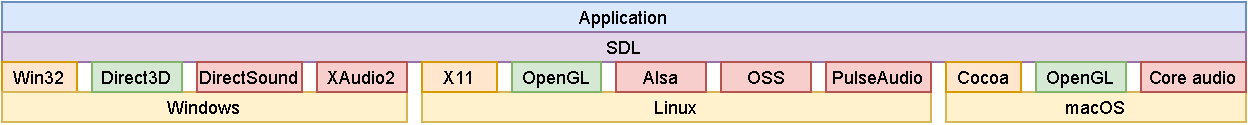
\includegraphics[width=\linewidth]{immagini/sdl}
	\caption{SDL: livelli di astrazione su diverse piattaforme}
	\label{fig:sdl}
\end{figure}


\subsection{Video}
Il MAME è in grado di emulare giochi sia 2D che 3D (es.: Tekken della Namco), ma poiché emula il monitor fisico ciò che viene inviato alle varie librerie grafiche è un insieme di primitive e texture da disegnare.

\begin{figure}[H]
	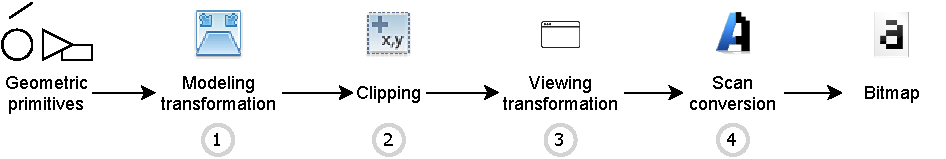
\includegraphics[width=\linewidth]{immagini/rendering_pipeline}
	\caption{Pipeline di rendering 2D}
	\label{fig:rendering_pipeline}
\end{figure}

Quando la finestra di gioco viene inizializzata, viene creato un contesto di rendering SDL per la finestra tramite la funzione \textit{CreateRenderer}. Per ogni frame della macchina che viene emulato c'è una fase di disegno usando \textit{SetRenderDrawColor}, \textit{RenderFillRect} e \textit{RenderDrawLine}, e poi tramite la funzione \textit{RenderPresent} viene mostrato il frame appena renderizzato sulla finestra.


\subsection{Audio}
Lorem ipsum dolor sit amet, consectetur adipiscing elit, sed do eiusmod tempor incididunt ut labore et dolore magna aliqua. Ut enim ad minim veniam, quis nostrud exercitation ullamco laboris nisi ut aliquip ex ea commodo consequat. Duis aute irure dolor in reprehenderit in voluptate velit esse cillum dolore eu fugiat nulla pariatur. Excepteur sint occaecat cupidatat non proident, sunt in culpa qui officia deserunt mollit anim id est laborum.



\section{Web APIs}
Le API Web sono un insieme di API e interfacce che comprendono la potente capacità di creazione di script del Web. A seguire quelli utilizzati in questo progetto\cite{Web_APIs}.

\subsection{WebSocket}
WebSocket è un protocollo di comunicazione del computer che fornisce canali di comunicazione full-duplex su una singola connessione TCP. È compatibile con HTTP perché l'handshake WebSocket utilizza l'intestazione di aggiornamento HTTP per passare dal protocollo HTTP al protocollo WebSocket. È supportato nativamente da tutti i browser e il suo utilizzo è simile ai normali socket sia sul lato client che su quello server. Per questi motivi è il protocollo di comunicazione generico più utilizzato sul web\cite{WebSocket_Web_APIs}.

\subsection{Canvas API}
L'API Canvas fornisce un mezzo per disegnare grafica tramite JavaScript, si concentra principalmente sulla grafica 2D ma quando viene utilizzata dall'API WebGL può disegnare grafica 2D e 3D con accelerazione hardware. È completamente supportato da tutti i browser\cite{Canvas_API}.

\subsection{WebGL API}
WebGL è un'API JavaScript, progettata e gestita dal gruppo no-profit Khronos, per il rendering di grafica 2D e 3D che consente l'utilizzo accelerato dalla GPU della fisica e dell'elaborazione e degli effetti delle immagini. WebGL 1.0 è supportato su tutti i browser, mentre WebGL 2.0 viene testato su Safari\cite{WebGL}.



\section{JavaScript libraries}
Per il front-end, sono state utilizzate tre librerie JavaScript open source per la gestione degli input e per la decodifica del filmato.

\subsection{JSMpeg}
JSMpeg è una libreria composta da un demuxer MPEG-TS, un decoder video MPEG1 e audio MP2, con un sistema di rendering basato sia su WebGL che su Canvas2D, ed un sistema di output audio basato su WebAudio. Consente lo streaming a bassa latenza ($\sim$50ms) tramite WebSocket, ed è rilasciata con licenza MIT\cite{JSMpeg}.

\subsection{Keypress}
Keypress è una libreria per la cattura dell'input da tastiera specializzata per l'uso in contesti videoludici, rilasciata con licenza Apache 2.0. Viene utilizzata per gestire l'input da tastiera nel front-end\cite{Keypress}.

\subsection{GameController.js}
GameController.js è una libreria che estende le Web API per il gamepad, è rilasciata con licenza MIT. Nel front-end viene utilizzata per gestire i gamepads, per consentire il multiplayer sullo stesso dispositivo\cite{gameController_js}.